%**************************************************************************************
% License:
% CC BY-NC-SA 4.0 (http://creativecommons.org/licenses/by-nc-sa/4.0/)
%**************************************************************************************

\documentclass[notes]{beamer}

\mode<presentation> {

\usetheme{Madrid}

% Burnt orange
\definecolor{burntorange}{rgb}{0.8, 0.33, 0.0}
\colorlet{beamer@blendedblue}{burntorange}
% Pale yellow
\definecolor{paleyellow}{rgb}{1.0, 1.0, 0.953}
\setbeamercolor{background canvas}{bg=paleyellow}
% Secondary and tertiary palette
\setbeamercolor*{palette secondary}{use=structure,fg=white,bg=burntorange!80!black}
\setbeamercolor*{palette tertiary}{use=structure,fg=white,bg=burntorange!60!black}

% To remove the navigation symbols from the bottom of all slides uncomment this line
%\setbeamertemplate{navigation symbols}{}
}

\usepackage{amsmath}
\DeclareMathOperator*{\argmin}{arg\,min}
\DeclareMathOperator*{\argmax}{arg\,max}
\usepackage{bm}
\usepackage{booktabs} % Allows the use of \toprule, \midrule and \bottomrule in tables
\usepackage{breqn}
\usepackage{cleveref}
\usepackage{graphicx} % for figures
\usepackage[labelsep=space,tableposition=top]{caption}
\renewcommand{\figurename}{Fig.} 
\usepackage{caption,subcaption}% http://ctan.org/pkg/{caption,subcaption}
\usepackage{xcolor}
\usepackage{hyperref}

\AtBeginSection[]{
	\begin{frame}{Outline}
		\tableofcontents[
		currentsection,      % highlight the current section
		hideallsubsections   % show only section titles
		]
	\end{frame}
}

%----------------------------------------------------------------------------------------
%	TITLE PAGE
%----------------------------------------------------------------------------------------
\title[Differentiable Simulation]{Differentiable Simulation: Making Physics Learnable} 
\author{Krishna Kumar} % name
\institute[UT Austin] % institution 
{
University of Texas at Austin \\
\medskip
\textit{
  \url{krishnak@utexas.edu}} % Your email address
}
\date{} % Date, can be changed to a custom date

\begin{document}

\begin{frame}
\titlepage % title page as the first slide
\end{frame}

\begin{frame}
 \frametitle{Overview}
 \tableofcontents
\end{frame}

%----------------------------------------------------------------------------------------
% slides
%----------------------------------------------------------------------------------------

\section{Introduction: From Neural Networks to Physics}

%------------------------------------------------
\begin{frame}
\frametitle{Learning Objectives}

\begin{itemize}
    \item Understand the paradigm shift from traditional simulation to differentiable simulation
    \item Learn how automatic differentiation enables gradient-based optimization in physics
    \item Master the JAX framework for high-performance scientific computing
    \item Implement a differentiable wave equation solver
    \item Apply differentiable simulation to Full Waveform Inversion (FWI)
\end{itemize}

\vspace{1cm}
\centering
\href{https://colab.research.google.com/github/kks32-courses/sciml/blob/main/lectures/03-diffsim/03-diffsim.ipynb}{\beamergotobutton{Open Notebook: Differentiable Simulation}}

\end{frame}

%------------------------------------------------
\begin{frame}
\frametitle{What is Differentiable Simulation?}

\textbf{Traditional Simulation:}
\begin{itemize}
    \item Given parameters → compute forward simulation
    \item Trial-and-error parameter search for inverse problems
    \item Expensive, often requires domain expertise
\end{itemize}

\vspace{1cm}

\begin{alertblock}{Differentiable Simulation Revolution}
If we can compute $\frac{\partial \text{simulation}}{\partial \text{parameters}}$, we can use gradient descent to find optimal parameters!
\end{alertblock}

\textbf{The Paradigm Shift:}
\begin{itemize}
    \item \textbf{Forward Problem}: Given parameters → predict observations
    \item \textbf{Inverse Problem}: Given observations → optimize parameters using gradients
\end{itemize}

\end{frame}

%------------------------------------------------
\begin{frame}
\frametitle{The Power of Automatic Differentiation}

\begin{columns}[T]
    \begin{column}{0.5\textwidth}
        \textbf{PyTorch Example:}
        \begin{itemize}
            \item Tracks all operations on tensors
            \item \texttt{.backward()} computes gradients
            \item Reverse-mode AD (backpropagation)
        \end{itemize}
        
        \vspace{0.5cm}
        
        \textbf{Simple loss function:}
        \begin{equation*}
        L = (ax + b - \text{target})^2
        \end{equation*}
    \end{column}
    \begin{column}{0.5\textwidth}
        \textbf{JAX Advantages:}
        \begin{itemize}
            \item Functional programming approach
            \item JIT compilation for speed
            \item Composable transformations
            \item \texttt{grad}, \texttt{jit}, \texttt{vmap}
        \end{itemize}
        
        \vspace{0.5cm}
        
        \textbf{Same computation in JAX:}
        \begin{equation*}
        \text{grad\_fn} = \text{grad}(\text{loss\_fn})
        \end{equation*}
    \end{column}
\end{columns}

\end{frame}

%------------------------------------------------
\section{JAX: The Scientific Computing Framework}

%------------------------------------------------
\begin{frame}
\frametitle{JAX Transformations: The Power of Composition}

\textbf{Key transformations work together:}

\begin{block}{Core Transformations}
\begin{itemize}
    \item \textbf{grad}: Automatic differentiation
    \item \textbf{jit}: Just-In-Time compilation
    \item \textbf{vmap}: Vectorization (automatic batching)
\end{itemize}
\end{block}

\textbf{Example: Polynomial with transformations}
\begin{equation*}
f(x) = x^4 - 3x^3 + 2x^2 - x + 1
\end{equation*}

\begin{itemize}
    \item \texttt{fast\_f = jit(f)} - Compiled version
    \item \texttt{df = grad(f)} - Gradient function
    \item \texttt{vectorized = vmap(f)} - Works on arrays
    \item \texttt{fast\_grad = jit(grad(f))} - Compiled gradient
\end{itemize}

\textbf{Performance gain:} 3× speedup with JIT compilation!

\end{frame}

%------------------------------------------------
\begin{frame}
\frametitle{JAX vs PyTorch for Physics}

\begin{columns}[T]
    \begin{column}{0.5\textwidth}
        \textbf{PyTorch:}
        \begin{itemize}
            \item Object-oriented design
            \item Mutable tensors
            \item Dynamic computation graphs
            \item Great for deep learning
        \end{itemize}
        
        \vspace{0.5cm}
        
        \textbf{Best for:}
        \begin{itemize}
            \item Neural network training
            \item Rapid prototyping
            \item Dynamic models
        \end{itemize}
    \end{column}
    \begin{column}{0.5\textwidth}
        \textbf{JAX:}
        \begin{itemize}
            \item Functional programming
            \item Immutable arrays
            \item Composable transformations
            \item NumPy-compatible API
        \end{itemize}
        
        \vspace{0.5cm}
        
        \textbf{Best for:}
        \begin{itemize}
            \item Scientific computing
            \item High-performance simulation
            \item Mathematical optimization
        \end{itemize}
    \end{column}
\end{columns}

\textbf{For physics simulations:} JAX's functional approach and JIT compilation provide significant advantages.

\end{frame}

%------------------------------------------------
\section{The 1D Wave Equation: Our Physics Model}

%------------------------------------------------
\begin{frame}
\frametitle{The 1D Acoustic Wave Equation}

\textbf{Governing equation:}
\begin{equation*}
\frac{\partial^2 u}{\partial t^2} = c^2 \frac{\partial^2 u}{\partial x^2}
\end{equation*}

Where:
\begin{itemize}
    \item $u(x,t)$ is the wavefield (pressure/displacement)
    \item $c(x)$ is the wave speed (what we want to estimate)
\end{itemize}

\vspace{1cm}

\textbf{Finite difference discretization:}
\begin{equation*}
u_{i}^{n+1} = 2u_{i}^{n} - u_{i}^{n-1} + \frac{c_i^2 \Delta t^2}{\Delta x^2}(u_{i+1}^{n} - 2u_{i}^{n} + u_{i-1}^{n})
\end{equation*}

\textbf{Initial conditions:} Gaussian source at $x = 0.5$
\begin{equation*}
u_0 = \exp(-5(x - 0.5)^2)
\end{equation*}

\end{frame}

%------------------------------------------------
\begin{frame}
\frametitle{The Forward Problem: Wave Propagation}

\begin{figure}[ht]
	\centering
	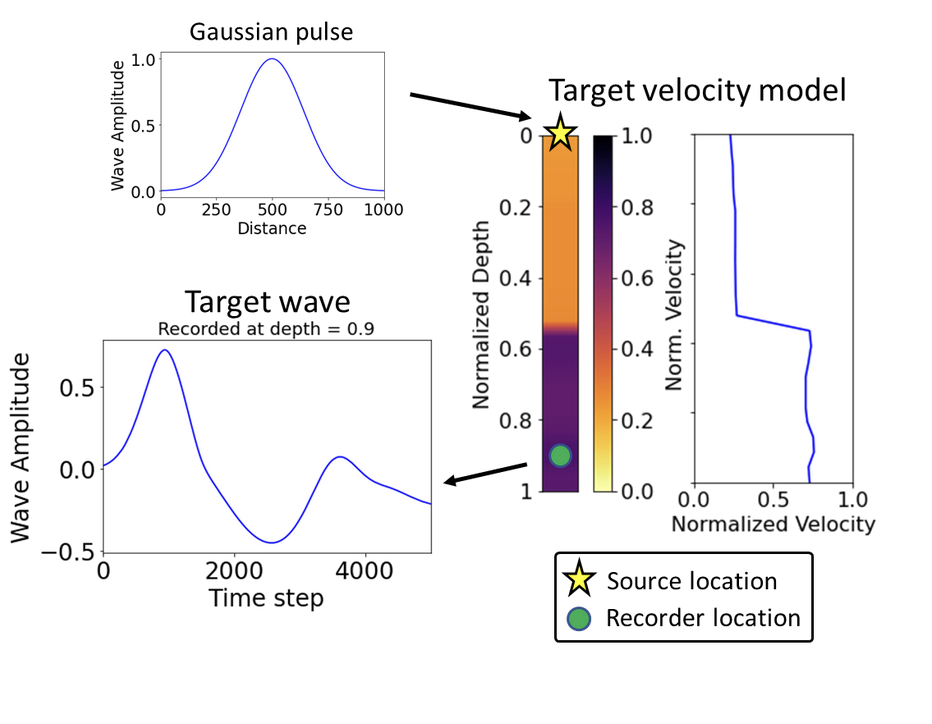
\includegraphics[width=0.8\textwidth]{figs/1dfwi.png}
	\caption*{1D Full Waveform Inversion setup showing wave propagation.}
\end{figure}

\textbf{Implementation details:}
\begin{itemize}
    \item 1000 spatial points on domain $[0, 1]$
    \item Time step $\Delta t = 5 \times 10^{-4}$
    \item CFL stability condition: $C = c\Delta t/\Delta x < 1$
    \item Boundary conditions: $u = 0$ at $x = 0, 1$
    \item 5000 time steps for complete simulation
\end{itemize}

\end{frame}

%------------------------------------------------
\begin{frame}
\frametitle{JAX Implementation: JIT-Compiled Solver}

\textbf{Key implementation features:}

\begin{block}{JIT Compilation}
\texttt{@jit} decorator compiles the entire time-stepping loop for high performance
\end{block}

\begin{block}{Functional Programming}
\begin{itemize}
    \item Pure functions with no side effects
    \item Immutable arrays (no in-place operations)
    \item \texttt{lax.fori\_loop} for compiled loops
\end{itemize}
\end{block}

\textbf{Central difference scheme:}
\begin{equation*}
u_2 = 2u_1 - u_0 + C^2(u_{1,j-1} - 2u_{1,j} + u_{1,j+1})
\end{equation*}

where $C^2 = c^2\Delta t^2/\Delta x^2$

\textbf{Boundary handling:} \texttt{jnp.roll} with explicit boundary setting

\end{frame}

%------------------------------------------------
\section{Full Waveform Inversion: The Inverse Problem}

%------------------------------------------------
\begin{frame}
\frametitle{Example 1: Constant Velocity Recovery}

\begin{figure}[ht]
	\centering
	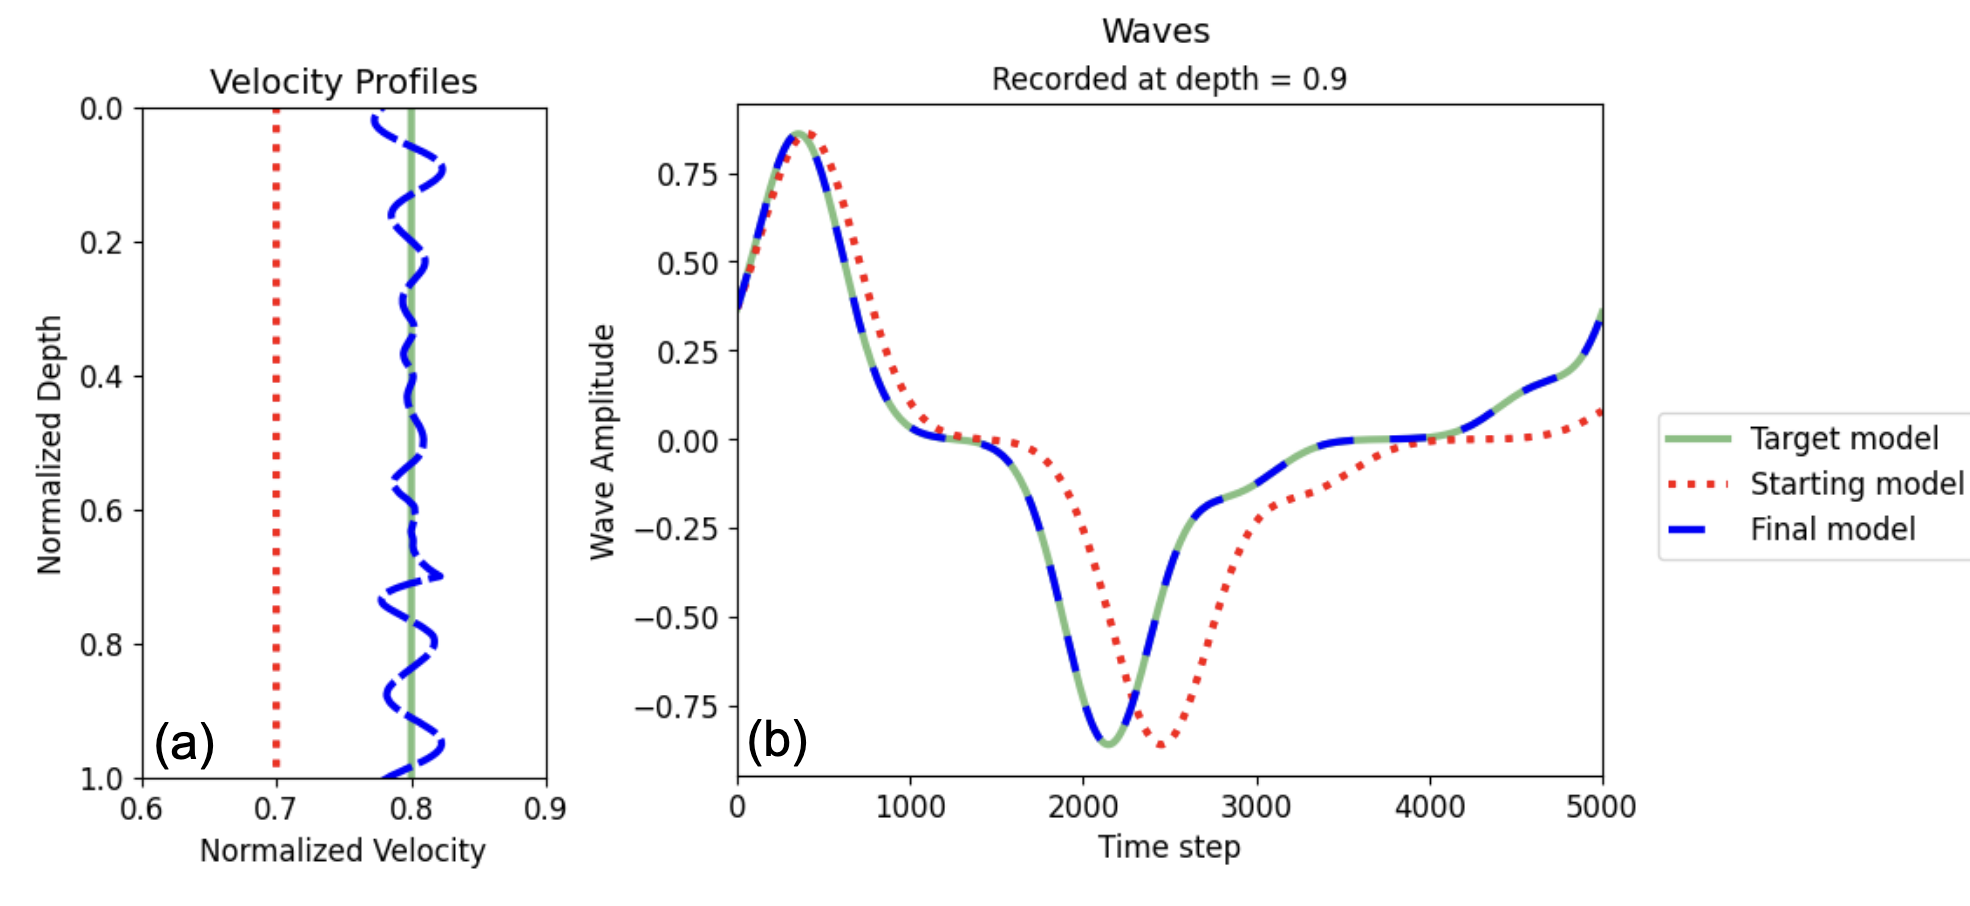
\includegraphics[width=0.8\textwidth]{figs/constant-profile-fwi.png}
	\caption*{Constant velocity recovery using gradient descent.}
\end{figure}

\textbf{Problem Setup:}
\begin{itemize}
    \item \textbf{Target}: $c = 1.0$ (constant velocity)
    \item \textbf{Initial guess}: $c = 0.8$
    \item \textbf{Optimization}: Adam optimizer with learning rate $10^{-3}$
\end{itemize}

\textbf{Results:}
\begin{itemize}
    \item Final velocity: $0.999937$ (error: $6.3 \times 10^{-5}$)
    \item Loss reduction: $840.8\times$
    \item Perfect recovery demonstrates gradient accuracy
\end{itemize}

\end{frame}

%------------------------------------------------
\begin{frame}
\frametitle{Example 2: Linear Velocity Profile}

\begin{figure}[ht]
	\centering
	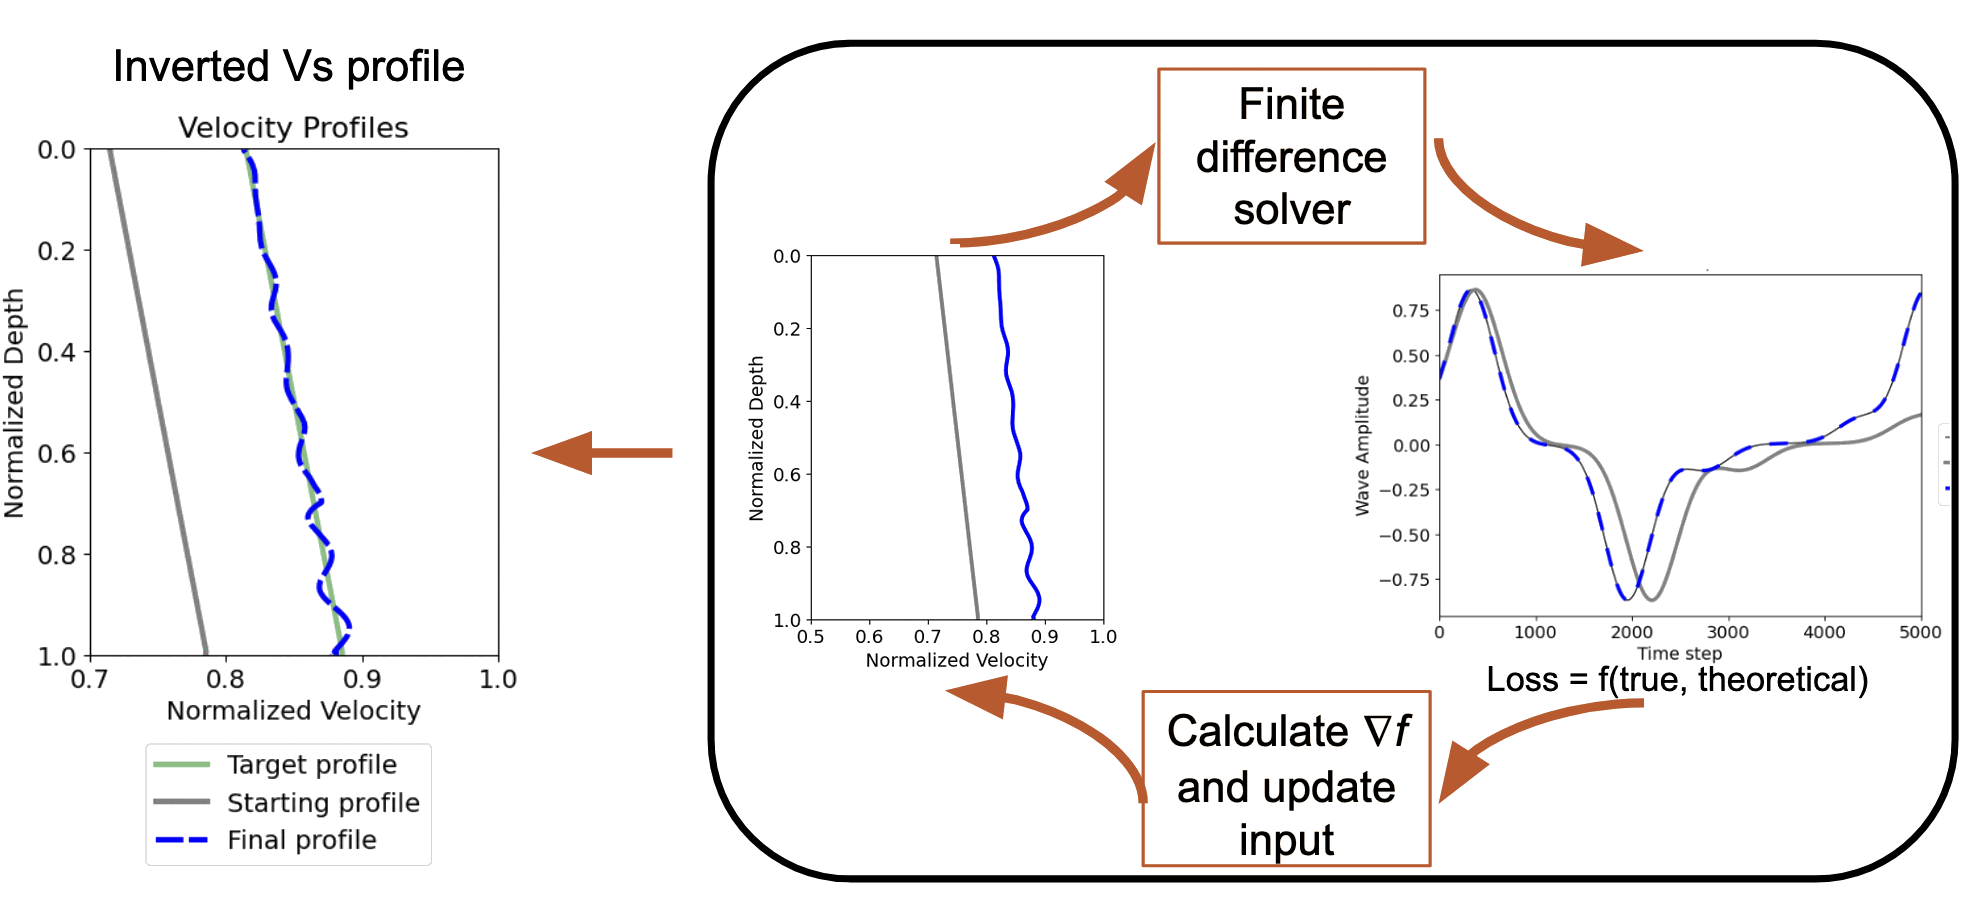
\includegraphics[width=0.8\textwidth]{figs/fwi-final.png}
	\caption*{Full waveform inversion animation showing optimization progress.}
\end{figure}

\textbf{Problem Setup:}
\begin{itemize}
    \item \textbf{Target}: $c(x) = 0.9 + 0.1x$ (linear increase)
    \item \textbf{Parameters}: 1000 spatial points to optimize
    \item \textbf{Challenge}: High-dimensional optimization landscape
\end{itemize}

\textbf{Algorithm Comparison:}
\begin{itemize}
    \item \textbf{Adam}: RMSE = $0.01696$
    \item \textbf{L-BFGS}: RMSE = $0.01420$ (1.2× better)
\end{itemize}

\end{frame}

%------------------------------------------------
\section{Advanced Optimization: Newton's Method and BFGS}

%------------------------------------------------
\begin{frame}
\frametitle{First-Order vs Second-Order Methods}

\begin{columns}[T]
    \begin{column}{0.5\textwidth}
        \textbf{First-Order (Adam):}
        \begin{equation*}
        x_{k+1} = x_k - \alpha \nabla f(x_k)
        \end{equation*}
        
        \textbf{Characteristics:}
        \begin{itemize}
            \item Uses only gradient information
            \item Robust to noise
            \item Memory: O(1) per parameter
            \item Good for large, noisy problems
        \end{itemize}
    \end{column}
    \begin{column}{0.5\textwidth}
        \textbf{Second-Order (L-BFGS):}
        \begin{equation*}
        x_{k+1} = x_k - H_k^{-1} \nabla f(x_k)
        \end{equation*}
        
        \textbf{Characteristics:}
        \begin{itemize}
            \item Uses curvature information
            \item Superlinear convergence
            \item Memory: O(m) history vectors
            \item Best for smooth functions
        \end{itemize}
    \end{column}
\end{columns}

\vspace{1cm}

\begin{alertblock}{L-BFGS Key Innovation}
Approximates inverse Hessian using gradient differences from recent iterations, avoiding expensive Hessian computation.
\end{alertblock}

\end{frame}

%------------------------------------------------
\begin{frame}
\frametitle{BFGS Update Formula}

\textbf{BFGS approximates the inverse Hessian iteratively:}

\begin{equation*}
H_{k+1} = (I - \rho_k s_k y_k^T) H_k (I - \rho_k y_k s_k^T) + \rho_k s_k s_k^T
\end{equation*}

Where:
\begin{itemize}
    \item $s_k = x_{k+1} - x_k$ (step difference)
    \item $y_k = \nabla f(x_{k+1}) - \nabla f(x_k)$ (gradient difference)  
    \item $\rho_k = \frac{1}{y_k^T s_k}$
\end{itemize}

\vspace{1cm}

\textbf{L-BFGS (Limited-memory BFGS):}
\begin{itemize}
    \item Stores only recent $m$ vector pairs $(s_k, y_k)$
    \item Suitable for large-scale problems
    \item Excellent for smooth optimization landscapes
\end{itemize}

\textbf{Our results:} L-BFGS achieved 20\% better accuracy than Adam for the smooth wave equation optimization.

\end{frame}

%------------------------------------------------
\section{Applications and Future Directions}

%------------------------------------------------
\begin{frame}
\frametitle{The Revolution: Physics as Learnable Components}

\textbf{What we've demonstrated:}

\begin{block}{Technical Achievements}
\begin{itemize}
    \item \textbf{Physics-Based Model}: Realistic wave equation with finite differences
    \item \textbf{Automatic Differentiation}: Exact gradients through entire simulation
    \item \textbf{Scalable Optimization}: 1 to 1000 parameters seamlessly
    \item \textbf{Algorithm Comparison}: Practical insights on optimizer choice
\end{itemize}
\end{block}

\begin{block}{Key Results}
\begin{itemize}
    \item \textbf{Constant velocity}: Perfect recovery with gradient descent
    \item \textbf{Linear profile}: High-fidelity reconstruction 
    \item \textbf{L-BFGS advantage}: Superior convergence for smooth landscapes
\end{itemize}
\end{block}

\textbf{The paradigm shift:} Physics simulations become \textbf{differentiable building blocks} for gradient-based optimization.

\end{frame}

%------------------------------------------------
\begin{frame}
\frametitle{Real-World Applications}

\begin{columns}[T]
    \begin{column}{0.5\textwidth}
        \textbf{Geophysics:}
        \begin{itemize}
            \item Subsurface imaging
            \item Earthquake location
            \item Earth structure inversion
            \item Oil and gas exploration
        \end{itemize}
        
        \vspace{0.5cm}
        
        \textbf{Medical Imaging:}
        \begin{itemize}
            \item Ultrasound tomography
            \item Photoacoustic imaging
            \item Tissue characterization
        \end{itemize}
    \end{column}
    \begin{column}{0.5\textwidth}
        \textbf{Engineering:}
        \begin{itemize}
            \item Structural health monitoring
            \item Non-destructive testing
            \item Design optimization
            \item Material characterization
        \end{itemize}
        
        \vspace{0.5cm}
        
        \textbf{Climate Science:}
        \begin{itemize}
            \item Atmospheric parameter estimation
            \item Ocean circulation models
            \item Weather prediction
        \end{itemize}
    \end{column}
\end{columns}

\vspace{1cm}

\textbf{Common theme:} Transform expensive inverse problems into efficient gradient-based optimization.

\end{frame}

%------------------------------------------------
\begin{frame}
\frametitle{Forward vs Inverse: The Complete Picture}

\begin{figure}[ht]
	\centering
	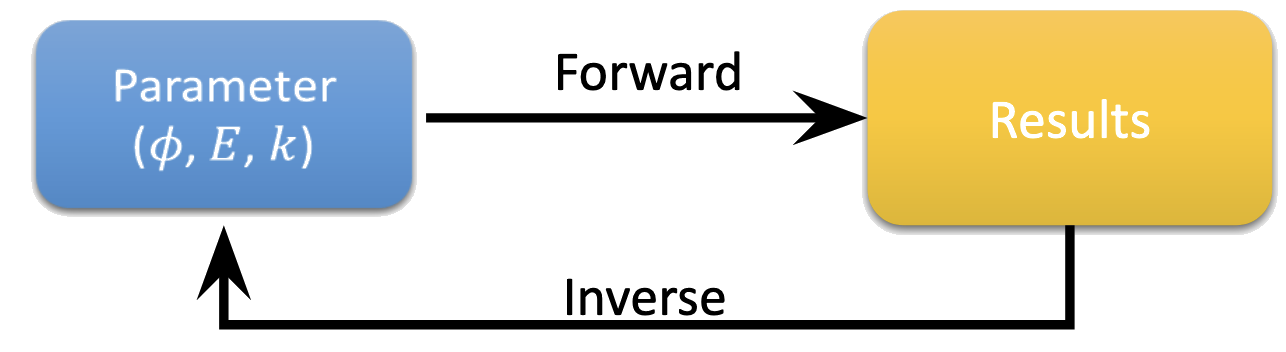
\includegraphics[width=0.8\textwidth]{figs/forward-inverse.png}
	\caption*{Forward and inverse problems in scientific computing.}
\end{figure}

\textbf{Traditional Approach:}
\begin{itemize}
    \item Forward problem: Well-posed, deterministic
    \item Inverse problem: Ill-posed, requires regularization
    \item Manual parameter tuning and domain expertise
\end{itemize}

\textbf{Differentiable Simulation:}
\begin{itemize}
    \item Automatic gradient computation through physics
    \item Principled optimization with advanced algorithms
    \item End-to-end learning from data to physics parameters
\end{itemize}

\end{frame}

%------------------------------------------------
\section{Summary and Future Directions}

%------------------------------------------------
\begin{frame}
\frametitle{Key Takeaways}

\begin{block}{1. Paradigm Shift}
\begin{itemize}
    \item Physics simulations become differentiable components
    \item Gradient-based optimization replaces trial-and-error
    \item JAX enables high-performance scientific computing
\end{itemize}
\end{block}

\begin{block}{2. Technical Implementation}
\begin{itemize}
    \item JIT compilation for performance
    \item Functional programming for correctness
    \item Composable transformations: \texttt{grad}, \texttt{jit}, \texttt{vmap}
\end{itemize}
\end{block}

\begin{block}{3. Optimization Insights}
\begin{itemize}
    \item L-BFGS excels for smooth physics problems
    \item Adam provides robustness for noisy/large-scale problems
    \item Second-order methods worth the complexity for precision
\end{itemize}
\end{block}

\end{frame}

%------------------------------------------------
\begin{frame}
\frametitle{Future Directions}

\textbf{Immediate Extensions:}
\begin{itemize}
    \item Multi-dimensional PDEs (2D/3D wave equations)
    \item Coupled multi-physics problems
    \item Stochastic differential equations
    \item Real-time optimization and control
\end{itemize}

\vspace{1cm}

\textbf{Advanced Topics:}
\begin{itemize}
    \item Physics-Informed Neural Networks (PINNs) integration
    \item Uncertainty quantification in inverse problems
    \item Multi-objective optimization with physical constraints
    \item Hybrid neural-physics models
\end{itemize}

\vspace{1cm}

\textbf{Next Steps:}
\begin{itemize}
    \item Explore the interactive projectile demo
    \item Try different velocity models and PDE types
    \item Implement regularization techniques
    \item Combine with deep learning approaches
\end{itemize}

\end{frame}

%------------------------------------------------
\begin{frame}
\frametitle{The Bigger Picture: Scientific Machine Learning}

\begin{center}
\textbf{Differentiable simulation bridges physics and machine learning}
\end{center}

\vspace{1cm}

\begin{columns}[T]
    \begin{column}{0.5\textwidth}
        \textbf{Traditional Scientific Computing:}
        \begin{itemize}
            \item Model-driven approach
            \item Physics-based equations
            \item Limited by computational cost
            \item Parameter sensitivity analysis
        \end{itemize}
    \end{column}
    \begin{column}{0.5\textwidth}
        \textbf{Machine Learning:}
        \begin{itemize}
            \item Data-driven approach
            \item Pattern recognition
            \item Scalable optimization
            \item Automatic differentiation
        \end{itemize}
    \end{column}
\end{columns}

\vspace{1cm}

\begin{alertblock}{The Synthesis}
Differentiable simulation combines the best of both worlds:
\begin{itemize}
    \item Physical constraints and interpretability
    \item Efficient gradient-based optimization
    \item End-to-end learning from observations to parameters
\end{itemize}
\end{alertblock}

\end{frame}

%------------------------------------------------
\begin{frame}
\frametitle{Questions?}

\centering
\Large Thank you!

\vspace{2cm}

\textbf{Contact:} \\
Krishna Kumar \\
\textit{krishnak@utexas.edu} \\
University of Texas at Austin

\vspace{1cm}

\textbf{Interactive Demo:} \\
\href{https://colab.research.google.com/github/kks32-courses/sciml/blob/main/lectures/03-diffsim/diffsim.ipynb}{\beamergotobutton{Differentiable Simulation Notebook}}

\end{frame}

\end{document}